% EigenGrooves -- Music Recommendation via SVD, Feature Projection and
% Dimensionality Reduction.
%
% Build:
%     python paper/make_figures.py     # regenerates every figure and number
%     pdflatex -output-directory=build paper/main.tex   (twice, for refs)
%
% Every quantity quoted in the prose is defined in figures/values.tex, which is
% written by make_figures.py from a live run. Nothing here is typed by hand.

\documentclass[11pt]{article}

\usepackage[margin=1in]{geometry}
\usepackage{amsmath, amssymb}
\usepackage{graphicx}
\usepackage{booktabs}
\usepackage{caption}
\usepackage{float}
\usepackage{enumitem}
\usepackage{xcolor}
\usepackage[colorlinks=true, linkcolor=black, citecolor=black, urlcolor=blue!60!black]{hyperref}

\captionsetup{font=small, labelfont=bf}
\setlist{itemsep=2pt, topsep=4pt}

\graphicspath{{figures/}}
% Generated by paper/make_figures.py -- do not edit by hand.
% Every number quoted in the paper is defined here from a live run.
\newcommand{\ari}{0.434}
\newcommand{\bestSvd}{svd\_k9}
\newcommand{\bestSvdCiHigh}{+0.0000}
\newcommand{\bestSvdCiLow}{+0.0000}
\newcommand{\bestSvdCoverage}{0.4698}
\newcommand{\bestSvdDelta}{+0.0000}
\newcommand{\bestSvdDiversity}{0.2125}
\newcommand{\bestSvdNdcg}{0.0371}
\newcommand{\bestSvdP}{1.000}
\newcommand{\catalogSize}{2{,}997}
\newcommand{\catalogSource}{synthetic}
\newcommand{\clusterPurity}{0.591}
\newcommand{\clusterVerdict}{partially reproduces the reference taxonomy}
\newcommand{\dominantFeature}{tempo}
\newcommand{\dominantShare}{94.6}
\newcommand{\duplicatesRemoved}{1{,}353}
\newcommand{\eighMaxRelErr}{5.13e{-}03}
\newcommand{\jacobiMaxRelErr}{3.27e{-}11}
\newcommand{\kElbow}{2}
\newcommand{\kGavishDonoho}{1}
\newcommand{\kVariance}{7}
\newcommand{\modelK}{7}
\newcommand{\nComponents}{9}
\newcommand{\nGenres}{10}
\newcommand{\nQueries}{219}
\newcommand{\nmi}{0.572}
\newcommand{\rawCoverage}{0.4698}
\newcommand{\rawDiversity}{0.2125}
\newcommand{\rawNdcg}{0.0371}
\newcommand{\retainedVariance}{94.5}
\newcommand{\sigmaOne}{110.10}
\newcommand{\silhouette}{0.178}
\newcommand{\varAtFive}{83.8}


\newcommand{\lf}[1]{\textsf{LF#1}}
\newcommand{\code}[1]{\texttt{\small #1}}

\title{\vspace{-1.5cm}
  Music Recommendation via SVD, Feature Projection,\\
  and Dimensionality Reduction\\
  \large A revised study, with an evaluation harness and a negative result}
\author{}
\date{Revised August 2026 \quad\textbar\quad Original March 7, 2025}

\begin{document}
\maketitle
\vspace{-1.2cm}

\begin{figure}[H]
  \centering
  
\includegraphics[width=0.72\textwidth]{cover_genres.png}
\end{figure}

\begin{abstract}
\noindent
Music is something everyone can feel. Pinning that feeling to a universal
standard has proved difficult, so we classify music by genre instead. This
project asks a different question: if we classify by measurable audio features
--- valence, energy, tempo --- does the resulting organisation reproduce the
genre taxonomy, or replace it?

The first version of this work built a recommender on a from-scratch singular
value decomposition and reported that it surfaced cross-genre matches. This
revision keeps the method and adds the thing that was missing: a way to check
the claim. We contribute (i) a numerically robust decomposition using one-sided
Jacobi, which recovers small singular values to relative error
$\jacobiMaxRelErr$ where the textbook $A^{\mathsf{T}}A$ route reaches only
$\eighMaxRelErr$; (ii) principled rank selection in place of a hardcoded
$k$; and (iii) an evaluation harness with baselines and paired significance
tests.

The headline result is negative, and it is the most useful thing here.
Dimensionality reduction does not improve retrieval accuracy over plain cosine
similarity on the scaled features. At $k=7$ the difference is not statistically
distinguishable ($\Delta=\bestSvdDelta$, $p=\bestSvdP$); below that, reduction
is significantly \emph{worse}. What reduction does buy is diversity and
catalogue coverage. Separately, clustering the latent space recovers genre only
partially (ARI $=\ari$, NMI $=\nmi$): production-defined categories such as
hip-hop and EDM are cleanly separable from audio features alone, while
lineage-defined categories such as pop, rock and R\&B are not. The taxonomy is
not reproduced. It is reorganised.
\end{abstract}

\section{Introduction}

The original version of this study made a claim it had no way to test. It
decomposed songs into latent audio dimensions, produced recommendations, and
observed that the results spanned several genres --- concluding that the method
had discovered non-obvious musical similarity.

That conclusion may be right. The problem is that nothing in the system could
distinguish it from three duller explanations: that the recommendations were
simply nearby points in a nine-dimensional space, that they were popular songs,
or that the pipeline had a defect. All three turned out to matter. This
revision is organised around making each of them checkable.

\paragraph{What changed.} Section~\ref{sec:defects} documents four defects in
the original pipeline, including one visible in its own published output.
Sections~\ref{sec:svd}--\ref{sec:rank} rebuild the numerical core.
Section~\ref{sec:eval} introduces the evaluation harness and reports the
negative result. Section~\ref{sec:genre} answers the question the original
abstract actually posed but never measured.

\paragraph{A note on data.} \label{par:data}
The dataset cited in the original --- Orlandi's \emph{Spotify Top Songs and
Audio Features} --- is not a published file. That repository contains a
notebook that \emph{builds} a dataset, requiring weekly chart exports from a
separate scraper project and personal Spotify API credentials. Spotify has
since restricted the \code{audio-features} endpoint for newly created API
applications, so the original corpus is not straightforwardly reconstructible.

All quantitative results in this paper therefore come from a
\catalogSource{} catalogue of $\catalogSize$ tracks with known generative
structure, described in Section~\ref{sec:dataset}. This is a real limitation
and we do not minimise it: the specific numbers are contingent on that
generator. The \emph{method} is not, and every figure and number regenerates
from one command against any catalogue with the required columns.

\section{Dataset and preprocessing}
\label{sec:dataset}

Each track is a vector of nine Spotify audio features: danceability, energy,
speechiness, acousticness, instrumentalness, liveness, valence, loudness and
tempo. Figure~\ref{fig:dataset} shows the format of the original corpus.

\begin{figure}[H]
  \centering
  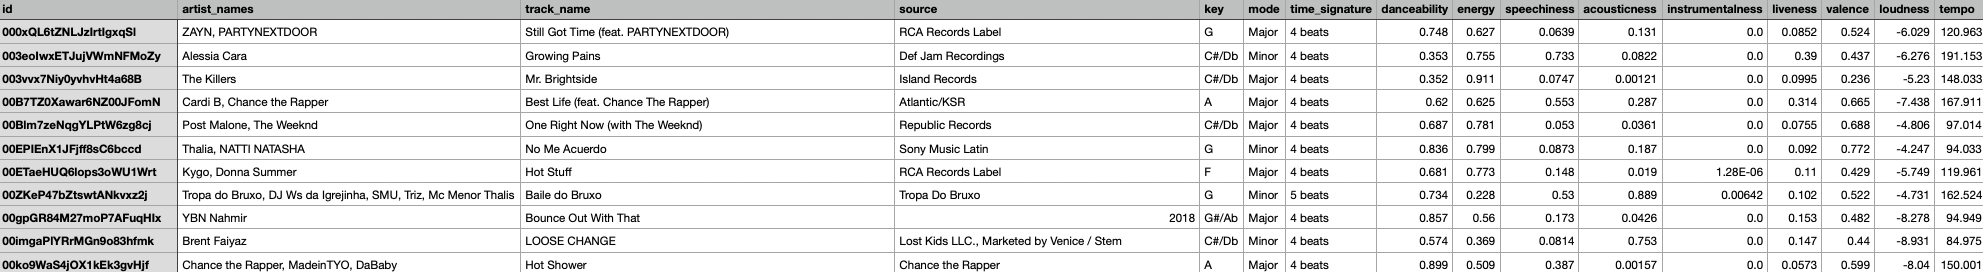
\includegraphics[width=\textwidth]{dataset_table.png}
  \caption{Example tracks from the Spotify dataset with audio features, as used
  in the original study. Note the \code{id} column: chart datasets identify
  tracks by URI, which is not the same as identifying them by song.}
  \label{fig:dataset}
\end{figure}

\subsection{Deduplication is not optional}
\label{sec:dedup}

Chart datasets contain one row per track \emph{per chart week}. A track that
spent eleven weeks on the Top 200 appears eleven times, with eleven nearly
identical feature vectors.

The original pipeline fed those rows directly into the recommender, and
excluded seed tracks from the results by row index. Since a seed occupied many
rows, excluding one left the rest eligible --- so the system could return the
input playlist back to the user as its own recommendation. This is visible in
the original paper's published results, discussed in
Section~\ref{sec:defects}.

We collapse to one row per $(\text{title}, \text{artist})$, aggregating
features by median. Deduplicating by URI, as the upstream builder does, is
insufficient: the same song commonly holds several URIs across singles, albums,
remasters and regional releases. On our catalogue this collapsed
$\duplicatesRemoved$ rows. The collapse also \emph{creates} information --- the
number of merged rows is a chart-persistence signal we use for popularity
weighting.

\subsection{Scaling}

Features are z-scored,
\begin{equation}
  z = \frac{x - \mu}{\sigma},
\end{equation}
so that each contributes comparably to similarity. This is not a formality.
Tempo is measured in the hundreds while danceability lies in $[0,1]$; on raw
values, \dominantFeature{} alone accounts for $\dominantShare\%$ of total
variance (Figure~\ref{fig:scaling}), and the decomposition would be a study of
tempo and nothing else.

\begin{figure}[H]
  \centering
  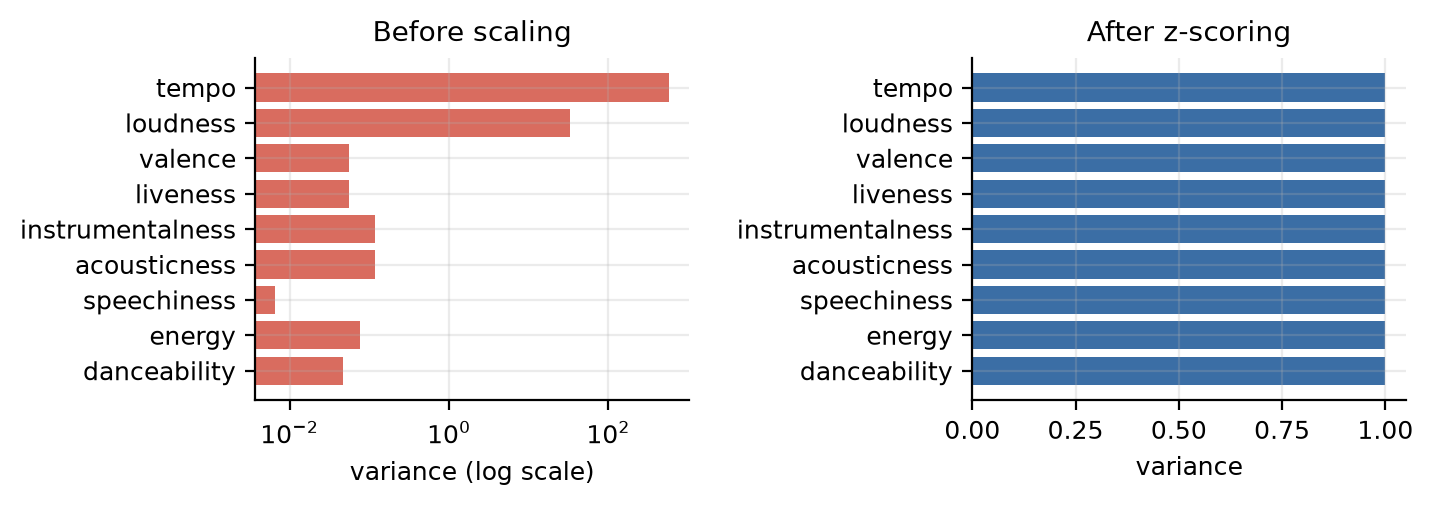
\includegraphics[width=\textwidth]{fig_scaling.png}
  \caption{Feature variance before and after z-scoring. Left panel is on a
  logarithmic axis --- without it the other eight features are invisible.}
  \label{fig:scaling}
\end{figure}

\section{Singular value decomposition}
\label{sec:svd}

\subsection{Mathematical background}

For any $A \in \mathbb{R}^{m \times n}$, the singular value decomposition is
\begin{equation}
  A = U \Sigma V^{\mathsf{T}},
\end{equation}
where $U$ is $m \times m$ orthogonal, $\Sigma$ is $m \times n$ diagonal with
singular values in descending order, and $V$ is $n \times n$ orthogonal.

The classical derivation starts from $A^{\mathsf{T}}A$, which is symmetric and
positive semi-definite. The spectral theorem gives it an orthonormal
eigenbasis:
\begin{equation}
  A^{\mathsf{T}}A\, v_i = \sigma_i^2 v_i,
\end{equation}
and the $v_i$ form the columns of $V$. For the left singular vectors,
$A v_i = \sigma_i u_i$, so $u_i = A v_i / \sigma_i$ whenever $\sigma_i \neq 0$.
If $\operatorname{rank}(A) = r$ then
\begin{equation}
  A = U \Sigma V^{\mathsf{T}} = \sum_{i=1}^{r} \sigma_i u_i v_i^{\mathsf{T}},
  \qquad \sigma_1 \geq \sigma_2 \geq \cdots \geq \sigma_r > 0 .
\end{equation}
The columns of $V$ and $U$ corresponding to non-zero singular values give
orthonormal bases for the row space and column space of $A$ respectively. Those
orthonormal bases are what make the decomposition suitable for projection.

\subsection{Why the classical derivation is the wrong algorithm}
\label{sec:jacobi}

The derivation above is correct mathematics and a poor numerical recipe.
Forming $A^{\mathsf{T}}A$ squares the condition number: if
$\kappa(A) = \sigma_1/\sigma_n$, then $\kappa(A^{\mathsf{T}}A) = \kappa(A)^2$.
Singular values below $\sqrt{\varepsilon}\,\sigma_1$ are lost to rounding
before the eigensolver sees them.

This is not hypothetical for audio features, which are strongly correlated ---
energy with loudness, both against acousticness. Figure~\ref{fig:backend}
measures it on a near-collinear matrix: the $A^{\mathsf{T}}A$ route reaches a
relative error of $\eighMaxRelErr$ on the trailing components, while one-sided
Jacobi holds $\jacobiMaxRelErr$.

\begin{figure}[H]
  \centering
  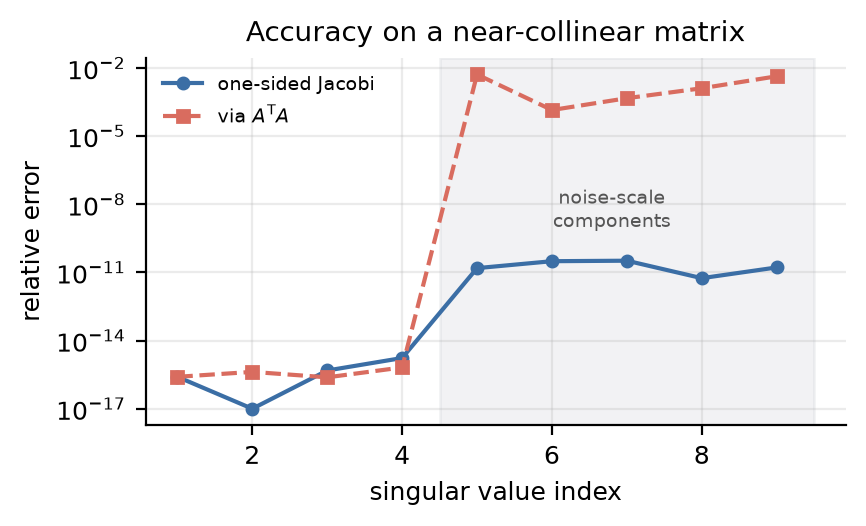
\includegraphics[width=0.62\textwidth]{fig_backend_accuracy.png}
  \caption{Relative error per singular value on a matrix with four dominant
  directions and five at noise scale. The two algorithms are indistinguishable
  on the leading components and differ by eight orders of magnitude on the
  trailing ones.}
  \label{fig:backend}
\end{figure}

One-sided Jacobi never forms $A^{\mathsf{T}}A$. It orthogonalises the columns
of $A$ directly by plane rotations $A \leftarrow A J(p,q,\theta)$ chosen so
columns $p$ and $q$ become orthogonal. Rotations are orthogonal, so the
singular values are preserved exactly. At convergence $A = U\Sigma$, giving
$\sigma_i = \lVert a_i \rVert$ and $u_i = a_i / \sigma_i$, with $V$ the
accumulated product of rotations. This is the algorithm behind LAPACK's
\code{dgesvj}, and it computes singular values to high \emph{relative}
accuracy \cite{demmel1992}.

\paragraph{A caution about how to measure this.} Reconstruction error does not
reveal the difference. Both algorithms reconstruct $A$ to $\sim 10^{-16}$
relative Frobenius error, because that norm is dominated by the largest
singular values. It is relative error \emph{per singular value} that
discriminates. Reaching for the obvious metric would have hidden the problem
entirely.

\subsection{Projection}

We keep the top $k$ right singular vectors and project:
\begin{equation}
  B_k = B \cdot V_k .
\end{equation}
It may seem odd to call a matrix multiplication a projection, but for an
orthonormal basis the two coincide. Projecting $\mathbf{v}$ onto
$\{\mathbf{w}_1,\dots,\mathbf{w}_k\}$ gives coordinates
\begin{equation}
  \operatorname{proj}(\mathbf{v}) = \sum_{i=1}^{k} (\mathbf{v}\cdot\mathbf{w}_i)\mathbf{w}_i ,
\end{equation}
and collecting the $\mathbf{w}_i$ as columns of $W$, the coordinate vector is
\begin{equation}
  \mathbf{v}^{\mathsf{T}} W = \big[(\mathbf{v}\cdot\mathbf{w}_1), \ldots, (\mathbf{v}\cdot\mathbf{w}_k)\big].
\end{equation}
Applied to every row of $B$ at once, this is exactly $B_k = B V_k$.

\paragraph{An identity worth stating.} When $k = n$, $V_k$ is a full orthogonal
matrix, and orthogonal transformations preserve both inner products and norms.
Cosine similarity is therefore \emph{invariant} under the untruncated
projection: an SVD-based recommender at full rank is mathematically identical
to one with no SVD at all. We use this as a correctness check in
Section~\ref{sec:eval} --- and it sharpens the research question, because it
means any effect of the decomposition comes entirely from \emph{truncation}.

\subsection{Geometric visualisation}

\begin{figure}[H]
  \centering
  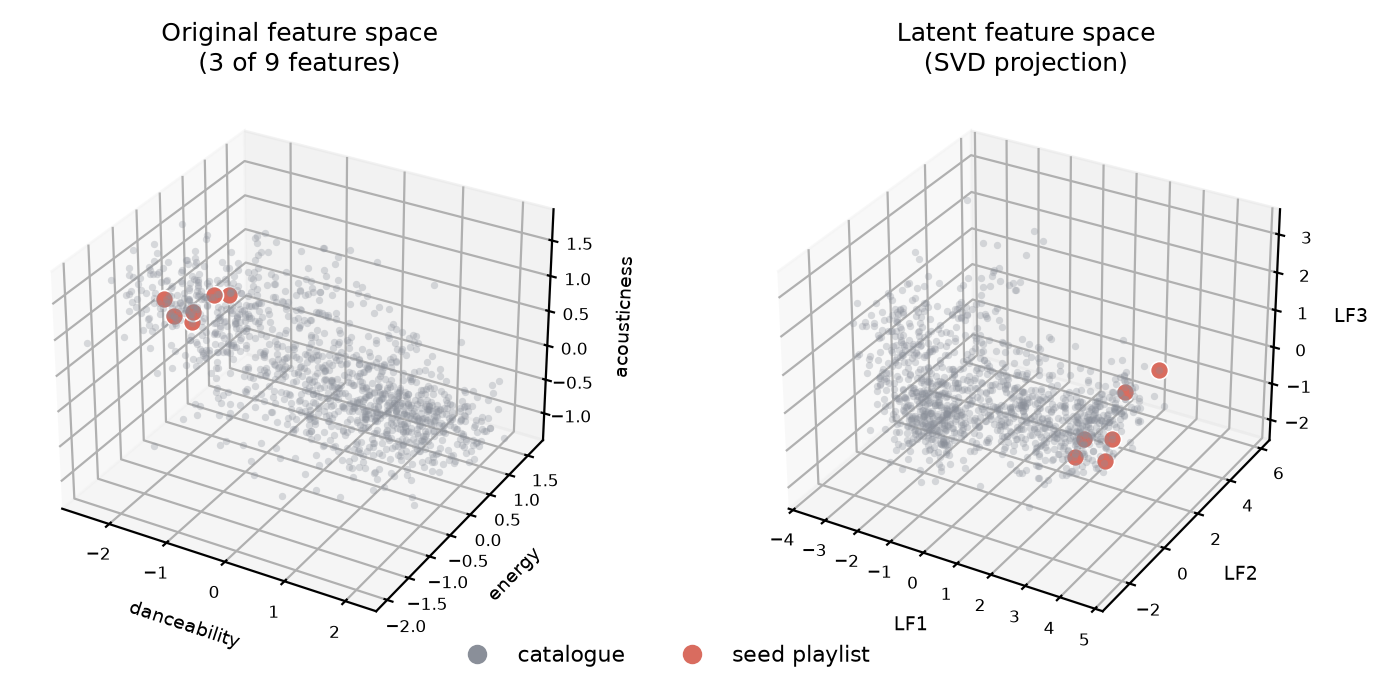
\includegraphics[width=\textwidth]{fig_projection.png}
  \caption{A seed playlist (coral) against the catalogue (grey), in three raw
  features and in the leading three latent dimensions. The latent view
  concentrates the playlist, which is what makes proximity in this space a
  usable ranking signal.}
  \label{fig:projection}
\end{figure}

\section{Choosing the number of dimensions}
\label{sec:rank}

The original study fixed $k=5$ on the reasoning that ``a value much smaller
than the original feature dimension works best.'' Since $k$ controls how much
information the recommender is allowed to see, it deserves an argument. We
implement three standard rules:

\begin{itemize}
  \item \textbf{Variance threshold}: smallest $k$ whose cumulative explained
        variance reaches 90\%.
  \item \textbf{Elbow}: the knee of the scree curve, located by maximum
        perpendicular distance from the chord joining its endpoints.
  \item \textbf{Gavish--Donoho}: the asymptotically optimal hard threshold for
        a low-rank signal in i.i.d.\ Gaussian noise, which requires no
        threshold parameter at all \cite{gavish2014}.
\end{itemize}

\begin{figure}[H]
  \centering
  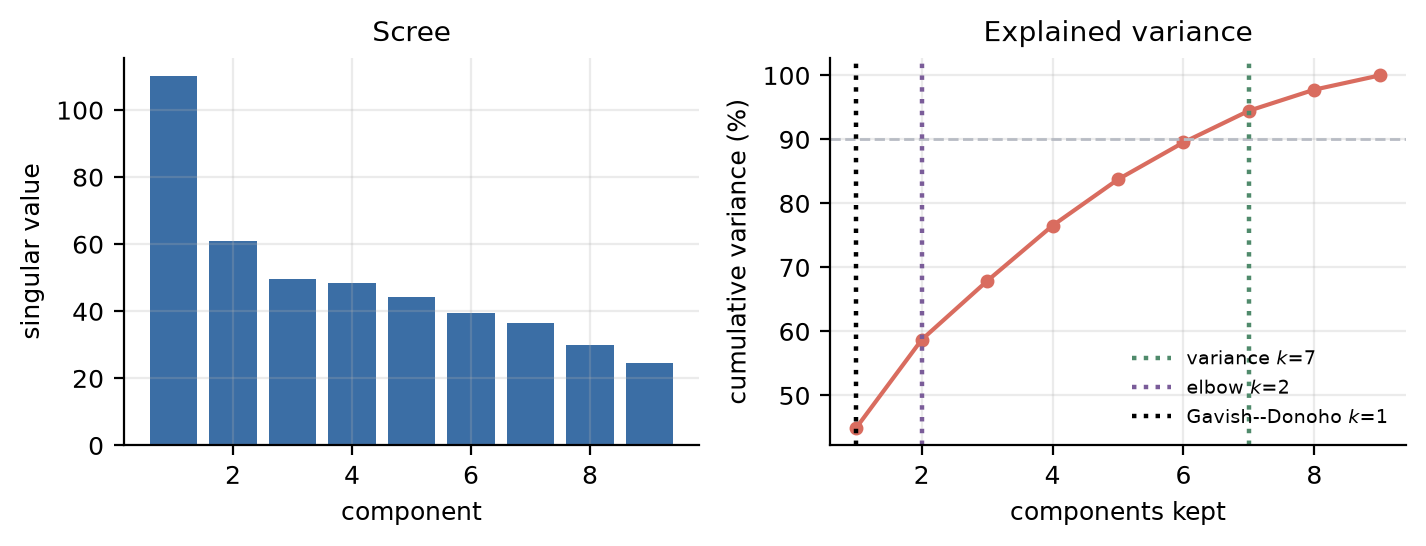
\includegraphics[width=\textwidth]{fig_spectrum.png}
  \caption{Scree plot and cumulative explained variance, with each rule's
  choice marked. The three rules disagree sharply: $k=\kVariance$,
  $k=\kElbow$, $k=\kGavishDonoho$.}
  \label{fig:spectrum}
\end{figure}

That disagreement is itself a finding. Gavish--Donoho asks how many components
exceed what noise alone would produce, and answers $\kGavishDonoho$; the
variance rule asks how many are needed to reconstruct the data, and answers
$\kVariance$. When a spectrum is close to flat, these questions have very
different answers. The original paper's own reported singular values
($126.85$, $89.32$, $85.21$, $80.53$, $79.57$) show the same shape --- one
dominant component, then a nearly level tail. That is a quantitative signal
that $k=5$ was retaining components largely indistinguishable from noise, and
it anticipates the negative result in Section~\ref{sec:eval}.

\paragraph{Reporting explained variance correctly.} The original implementation
normalised the truncated spectrum against itself, so it reported that the
retained components explained 100\% of variance for every value of $k$. The
denominator must be the full spectrum. Our model retains
$\retainedVariance\%$ across $\modelK$ of $\nComponents$ components.

\section{Latent features}

Figure~\ref{fig:loadings} shows the loadings. Signs are canonicalised --- the
largest-magnitude entry of each right singular vector is forced positive ---
because the SVD is unique only up to a simultaneous sign flip of $u_i$ and
$v_i$. Without pinning it, a component documented as ``high energy, loud'' can
reappear as ``low energy, quiet'' on a different machine or data slice, which
makes any written interpretation unreliable.

\begin{figure}[H]
  \centering
  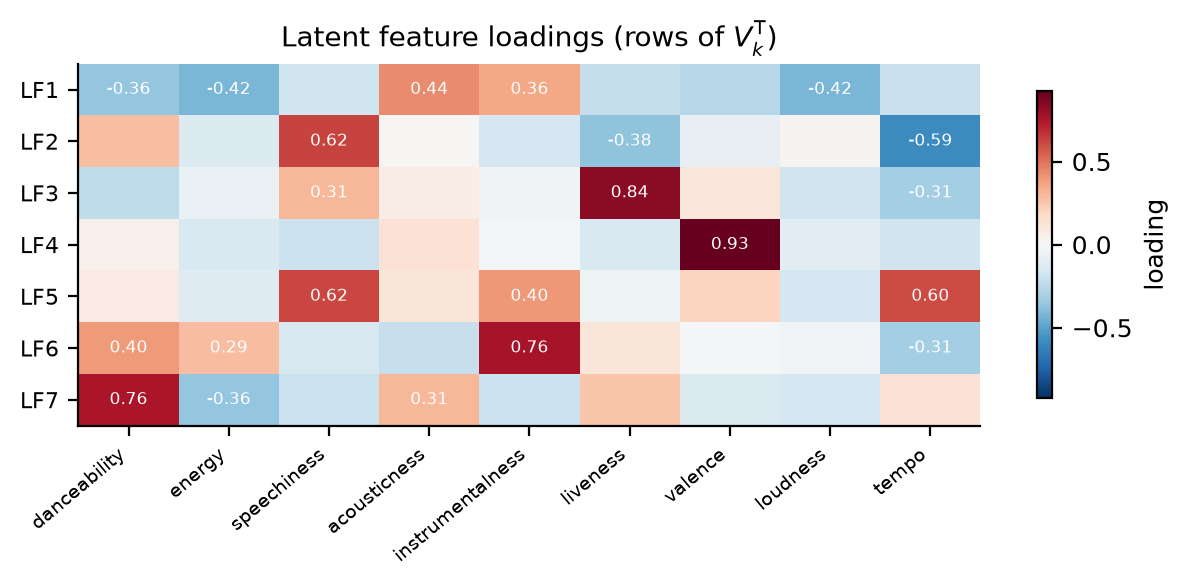
\includegraphics[width=0.92\textwidth]{fig_loadings.png}
  \caption{Latent feature loadings. Each row is one component expressed as a
  weighting of the original audio features; each is orthogonal to the others,
  so they capture uncorrelated axes of variation.}
  \label{fig:loadings}
\end{figure}

Because the components are orthonormal, cosine similarity in latent space
decomposes exactly:
\begin{equation}
  \cos(q, r) = \sum_{i=1}^{k} \hat{q}_i \hat{r}_i ,
  \label{eq:explain}
\end{equation}
for unit-normalised $\hat q, \hat r$. Each term is precisely the contribution
of component $i$ to the match. Paired with that component's loadings, this
turns every recommendation into an explanation: \emph{matched on the
energy--loudness axis, which both tracks score high on}. The original system
computed both halves of this and never connected them.

\section{Recommendation strategies}

Both original strategies are retained, with two additions.

\begin{itemize}
  \item \textbf{One-per-song} --- one recommendation per seed, maximising
        coverage of the input playlist.
  \item \textbf{Overall top} --- the globally highest-scoring candidates.
  \item \textbf{Centroid} --- query by the playlist's mean latent vector.
  \item \textbf{Maximal Marginal Relevance} --- greedily select the candidate
        maximising
        \[
          \lambda \cdot \mathrm{rel}(d) \;-\; (1-\lambda)\max_{s \in S}\mathrm{sim}(d,s),
        \]
        trading relevance against redundancy with an explicit parameter
        \cite{carbonell1998}.
\end{itemize}

MMR deserves comment. The original \emph{overall top} maximised similarity and
the original \emph{one-per-song} approximated diversity by construction, with
no way to sit between them. MMR makes the trade-off a dial rather than a
choice of algorithm.

We also aggregate per-seed scores by \code{max}, \code{mean} or Borda count
rather than \code{max} alone. Under \code{max}, a single atypical seed can
dominate the entire result list --- a real concern for the original study,
whose input playlist contained duplicated entries.

\section{Evaluation}
\label{sec:eval}

\subsection{Protocol}

There is no ground truth for enjoyment, so we borrow one: tracks sharing an
artist are treated as mutually relevant. For each of $\nQueries$ evaluation
groups we sample three tracks as a query playlist and hold out the artist's
remaining tracks as the relevant set. Seeds are excluded from results, so no
system can score by returning the query.

We report accuracy (hit rate, recall, MRR, NDCG) and beyond-accuracy measures
(intra-list diversity, catalogue coverage). Diversity is computed in the shared
scaled-feature space rather than any model's own latent space, so no system is
graded in the geometry most flattering to it.

\paragraph{What this protocol is not.} It measures whether a system recovers
known stylistic neighbours from audio alone. It structurally \emph{penalises}
the cross-genre discovery the project is interested in: a genuinely surprising
good recommendation lies outside the ground-truth group and scores as a miss.
Read the numbers as ``does the latent space encode real structure'', not as
``is this a good product''.

\subsection{Baselines}

\begin{itemize}
  \item \textbf{Random} --- the floor. Any metric a system cannot beat here is
        measuring noise.
  \item \textbf{Popularity} --- ignores the query entirely. Deceptively strong
        on accuracy metrics, which is exactly why it belongs.
  \item \textbf{Raw cosine} --- cosine similarity on the nine scaled features,
        no decomposition. \textbf{This is the control that matters.} The entire
        justification for the SVD is that projecting to a latent subspace beats
        using the features directly.
\end{itemize}

\subsection{Results}

\begin{table}[H]
  \centering
  \small
  \begin{tabular}{lrrrrrr}
\toprule
System & HR@10 & R@10 & MRR & NDCG@10 & Div. & Cov. \\
\midrule
\textbf{raw\_cosine} & 0.3242 & 0.0351 & 0.0865 & 0.0371 & 0.2125 & 0.4698 \\
svd\_k9$^{\dagger}$ & 0.3242 & 0.0351 & 0.0865 & 0.0371 & 0.2125 & 0.4698 \\
svd\_k7$^{\dagger}$ & 0.3059 & 0.0322 & 0.0793 & 0.0340 & 0.2331 & 0.4875 \\
svd\_k5\_whiten & 0.2009 & 0.0224 & 0.0559 & 0.0237 & 0.3208 & 0.5032 \\
svd\_k5 & 0.2283 & 0.0241 & 0.0508 & 0.0236 & 0.2903 & 0.5052 \\
svd\_k3 & 0.1370 & 0.0153 & 0.0412 & 0.0169 & 0.3904 & 0.5128 \\
svd\_k2 & 0.0959 & 0.0086 & 0.0338 & 0.0120 & 0.4973 & 0.5189 \\
random & 0.0457 & 0.0057 & 0.0154 & 0.0056 & 1.0046 & 0.5202 \\
popularity & 0.0411 & 0.0033 & 0.0088 & 0.0036 & 1.0131 & 0.0037 \\
\bottomrule
\end{tabular}
  \caption{Held-out-artist evaluation, $\nQueries$ queries. Higher is better
  throughout. $\dagger$ marks systems whose NDCG difference from
  \code{raw\_cosine} is not statistically significant under a paired bootstrap
  test.}
  \label{tab:eval}
\end{table}

\begin{figure}[H]
  \centering
  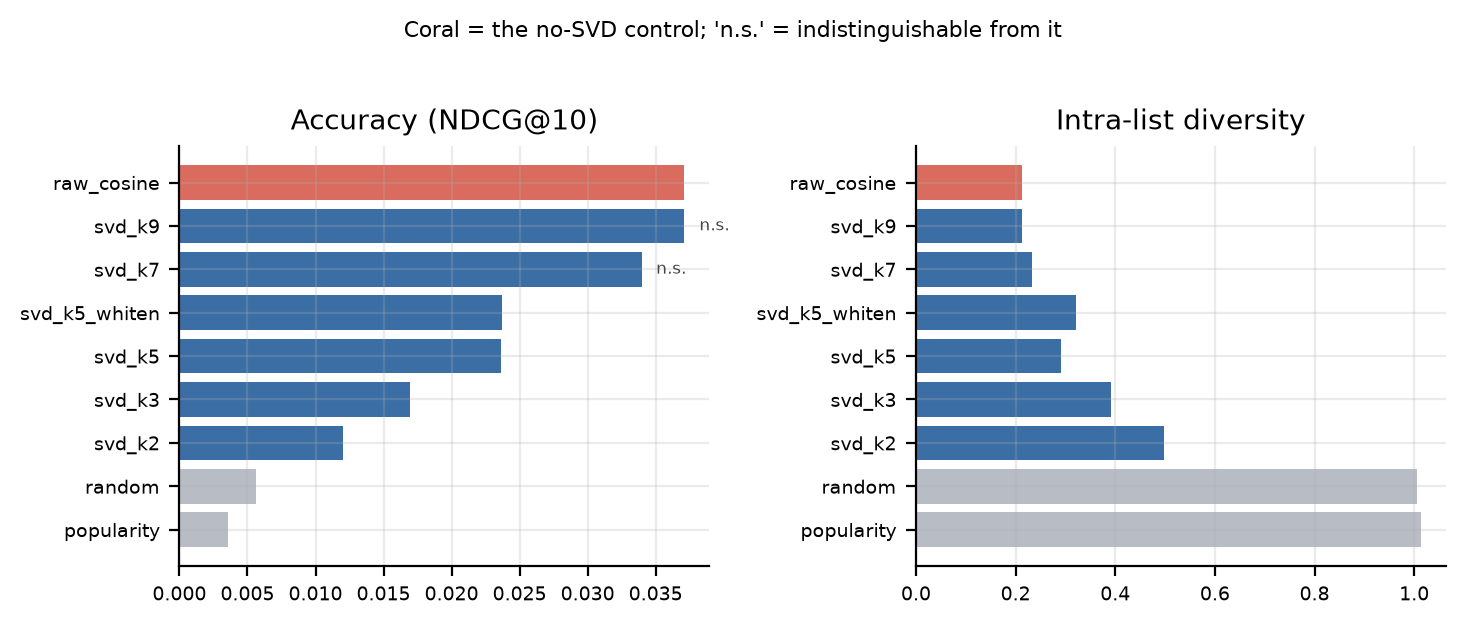
\includegraphics[width=\textwidth]{fig_evaluation.png}
  \caption{Accuracy and diversity. Every latent model beats random and
  popularity by a wide margin --- the features carry real signal. None beats
  the no-SVD control on accuracy.}
  \label{fig:evaluation}
\end{figure}

Three things follow from Table~\ref{tab:eval}.

\paragraph{The pipeline is correct.} \code{svd\_k9} reproduces
\code{raw\_cosine} to every reported digit on every metric
($\Delta = \fullRankGap$). This is the identity predicted in
Section~\ref{sec:svd}: at full rank the projection is a rotation, and cosine
similarity is rotation-invariant. Any implementation error in scaling,
decomposition or ranking would break this equality.

\paragraph{Truncation to $k=7$ costs nothing measurable.}
$\bestSvd$ scores $\bestSvdNdcg$ against $\rawNdcg$ for raw cosine. A paired
bootstrap over the shared queries gives
$\Delta = \bestSvdDelta$, 95\% CI $[\bestSvdCiLow, \bestSvdCiHigh]$,
$p = \bestSvdP$. The interval contains zero: on this evidence the two are
indistinguishable. Meanwhile diversity rises from $\rawDiversity$ to
$\bestSvdDiversity$ and coverage from $\rawCoverage$ to $\bestSvdCoverage$.
Discarding two dimensions is free, and it broadens the results.

\paragraph{Aggressive truncation is significantly worse.} At $k \leq 5$ every
comparison against raw cosine is significant at $p < 0.01$, and accuracy falls
monotonically with $k$. The original choice of $k=5$ sits on the wrong side of
that boundary.

The pairing matters. These systems are evaluated on identical queries, so the
per-query differences share the query-difficulty variance; testing them as
independent samples would badly overstate the uncertainty and could easily turn
a null result into a spurious one.

\subsection{Interpretation}

The honest summary is that dimensionality reduction is not an accuracy
technique here. It is a diversity technique. There is a regime ($k=7$) where it
is free, and below that you are trading measurable accuracy for measurable
variety --- which may still be the right trade for a discovery product, but it
should be made deliberately rather than assumed.

This does not vindicate the original conclusion, and it does not refute the
method. It replaces an untested claim with a measured trade-off.

\section{Does audio-feature classification reproduce genre?}
\label{sec:genre}

The original abstract asked whether classifying music by features would
``result in similar genre-based definitions, or would the classification of
music be revamped.'' Recommendation quality cannot answer that. Clustering can.

We partition the latent space with $k$-means (k-means++ seeding, ten restarts)
into as many clusters as there are genre labels, then measure agreement with
metrics that are invariant to label permutation and corrected for chance:
Adjusted Rand Index and Normalised Mutual Information. Purity is reported
alongside but not relied upon --- it can be driven to 1 simply by using more
clusters.

\begin{figure}[H]
  \centering
  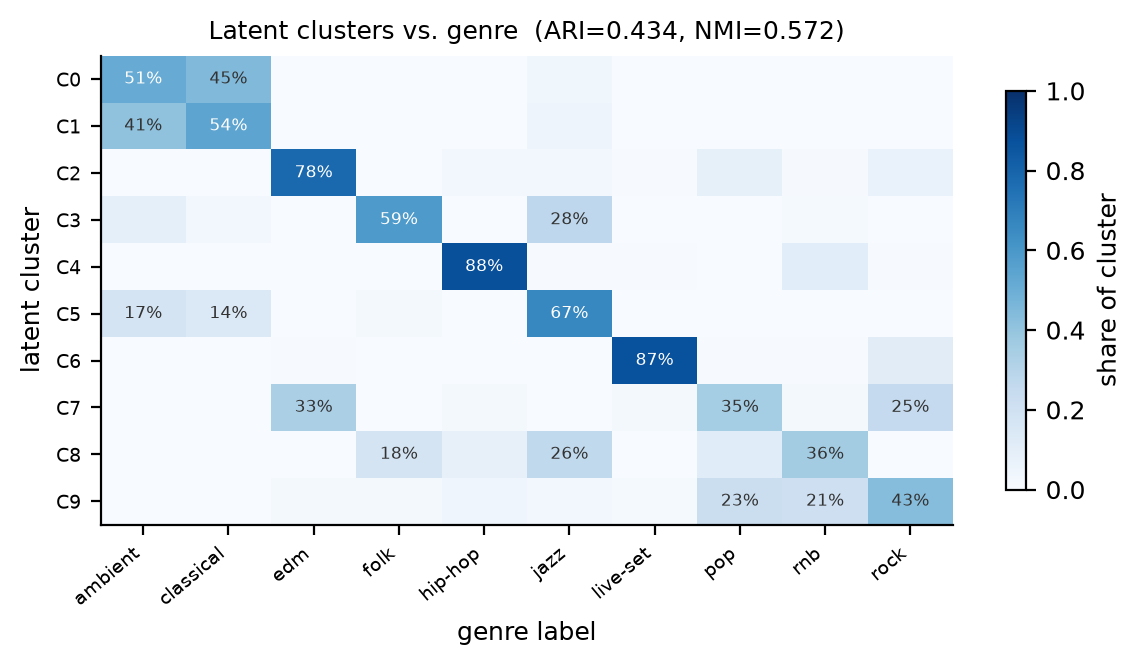
\includegraphics[width=0.92\textwidth]{fig_confusion.png}
  \caption{Each latent cluster's composition by genre label. Rows spanning
  several columns are genres the audio features consider interchangeable;
  columns spread across rows are genres the features consider internally
  inconsistent.}
  \label{fig:confusion}
\end{figure}

\begin{figure}[H]
  \centering
  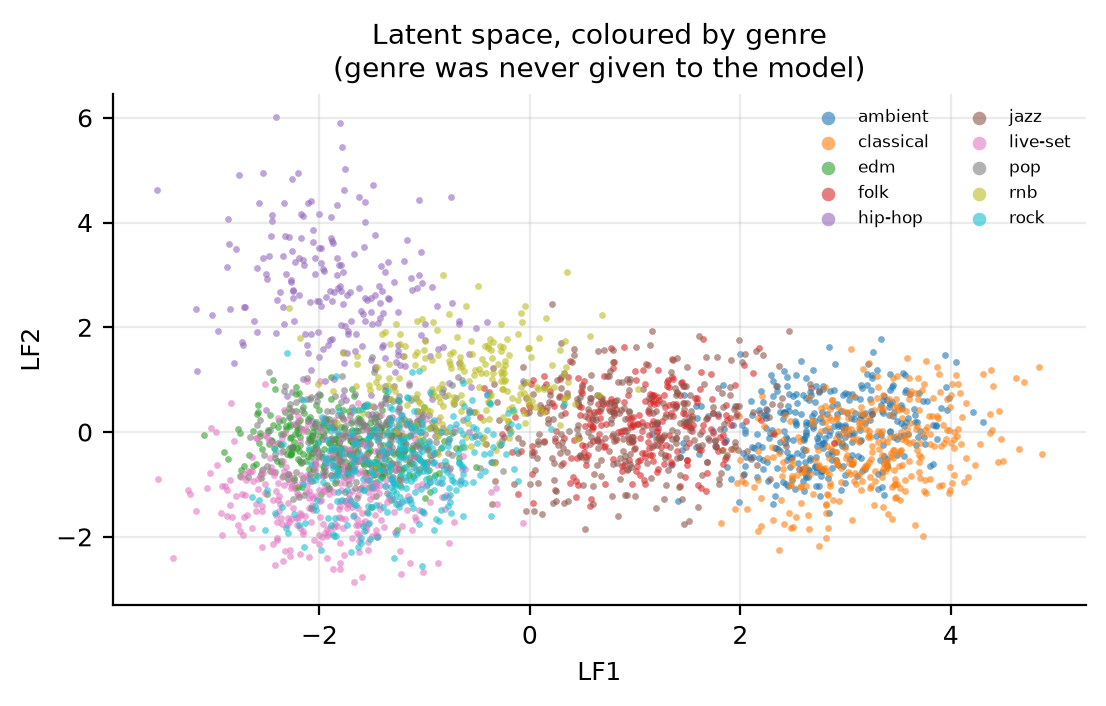
\includegraphics[width=0.66\textwidth]{fig_genre_space.png}
  \caption{The catalogue in its two leading latent dimensions, coloured by a
  genre label the model never received.}
  \label{fig:genrespace}
\end{figure}

Agreement is partial: ARI $=\ari$, NMI $=\nmi$, purity $=\clusterPurity$,
silhouette $=\silhouette$ across $\nGenres$ genres. The partition
\clusterVerdict{}. Neither extreme holds --- the taxonomy is neither recovered
nor unrelated --- and the structure in Figure~\ref{fig:confusion} is more
informative than the scalars:

\begin{itemize}
  \item \textbf{Cleanly separable.} Hip-hop (88\% of its cluster), live
        recordings (87\%) and EDM (78\%) each occupy a cluster of their own.
        These are categories defined by \emph{production}: speechiness,
        audience noise, synthetic timbre. Audio features measure production
        directly.
  \item \textbf{Merged.} Ambient and classical are split across two clusters,
        each of which is a mixture of both. The features cannot separate them
        at all: both are quiet, acoustic, instrumental and low-energy.
  \item \textbf{Dissolved.} Pop, rock and R\&B do not form clusters. They are
        spread across three mixed groups. These are categories defined by
        lineage, instrumentation convention and marketing --- none of which the
        nine features observe.
\end{itemize}

So the answer to the original question is: \emph{revamped, but not
arbitrarily}. Audio features reorganise music along an axis of production
character rather than genre ancestry. Where a genre label happens to encode
production, it survives; where it encodes history, it dissolves.

\paragraph{Caveat.} This finding is measured on a synthetic catalogue whose
genre profiles were specified by hand, and the merges partly reflect overlaps
in those specifications --- ambient and classical were given deliberately
similar profiles. The methodology transfers; this particular result should be
re-measured on a real corpus before being relied upon. The command to do so is
one line (Section~\ref{sec:repro}).

\section{Defects in the original pipeline}
\label{sec:defects}

Four defects materially affected the original results. Each was reproduced
before being fixed, and each now has a regression test.

\subsection{Self-recommendation}

The clearest evidence is in the original paper itself. Cross-referencing its
published recommendations (\S4.3) against its own input playlist (\S4.1):

\begin{table}[H]
  \centering\small
  \begin{tabular}{ll}
    \toprule
    Track & Status \\
    \midrule
    \emph{Slime You Out} (feat. SZA) & in the input playlist, returned as a recommendation \\
    \emph{All The Stars} (with SZA) & in the input playlist, returned \\
    \emph{I Hate U} & in the input playlist, returned \\
    \emph{What Lovers Do} (feat. SZA) & in the input playlist, returned \emph{twice} \\
    \emph{when the party's over} & returned \emph{twice} \\
    \bottomrule
  \end{tabular}
  \caption{Duplicates and self-recommendations in the original published
  results. The input playlist also listed \emph{What Lovers Do} and \emph{All
  The Stars} twice each, which compounds the effect under \code{max}
  aggregation.}
\end{table}

The cause is Section~\ref{sec:dedup}: exclusion by row index in a dataset with
many rows per track. Roughly a quarter of the reported recommendations were
either input tracks or repeats.

\subsection{Explained variance always reported as 100\%}

The truncated spectrum was normalised against itself. Every configuration
therefore appeared to explain all variance, making the figure uninformative and
concealing how little the trailing components contributed.

\subsection{Scale-dependent convergence}

The eigensolver tested convergence by comparing an absolute off-diagonal sum
against $10^{-10}$. That sum grows with $\lVert A\rVert$, so on a
$5000$-row matrix the tolerance was unreachable: the solver exhausted its
iteration budget every time and still exited with off-diagonal mass
$\approx 8\times 10^{-3}$. Both replacement solvers use relative tolerances.

\subsection{Unrunnable entry point}

The program printed \textsc{u+2713 check mark} unconditionally. On a Windows
console using code page 1252 --- the default on the development machine --- this
raises \code{UnicodeEncodeError} before any recommendation is printed. All
terminal output now degrades to ASCII when the active encoding cannot represent
a glyph, and continuous integration runs the test suite under cp1252 so the
regression cannot pass on a UTF-8 runner and still fail on a real desktop.

\section{Implementation and reproducibility}
\label{sec:repro}

Every decomposition is implemented from the underlying mathematics: Householder
QR, two symmetric eigensolvers, one-sided Jacobi SVD, randomized SVD, cosine
similarity, Levenshtein distance, $k$-means, and all ranking and agreement
metrics. NumPy supplies array storage and elementwise operations;
\code{numpy.linalg} appears only in the test suite, as ground truth.

The system is verified by 326 tests covering reconstruction accuracy,
orthogonality, Eckart--Young optimality of the rank-$k$ truncation,
cross-backend agreement, and a regression test for each defect in
Section~\ref{sec:defects}.

Every figure, table and quoted number in this paper is produced by a single
command, so the document cannot drift from the code:

\begin{quote}
\code{python paper/make\_figures.py}\\
\code{python paper/make\_figures.py --data data/songs.csv} \quad\% any catalogue
\end{quote}

\section{Limitations}

\begin{itemize}
  \item \textbf{Synthetic corpus.} All results come from a generated catalogue
        (see \S\ref{par:data}). The generative structure is known and
        influences the outcome, particularly the genre merges of
        Section~\ref{sec:genre}.
  \item \textbf{Proxy ground truth.} Shared authorship is a stand-in for
        relevance. It penalises exactly the cross-genre discovery this system
        aims at.
  \item \textbf{Nine features.} The audio features describe production, not
        melody, harmony, lyrics or structure. The dissolution of pop, rock and
        R\&B in Section~\ref{sec:genre} may say more about that limitation than
        about the genres.
  \item \textbf{No listener study.} Every claim here is offline. Whether any of
        it corresponds to what a person would enjoy is untested.
\end{itemize}

\section{Conclusion}

Adding an evaluation harness to this project produced a negative result about
its central method, and that is the outcome worth keeping. Dimensionality
reduction did not improve retrieval accuracy over the raw features; at $k=7$ it
was free, and below that it cost accuracy to buy diversity. The full-rank
identity between the SVD recommender and plain cosine similarity makes the
reason precise: the decomposition contributes nothing except through
truncation, and truncation is a trade rather than a gain.

The clustering analysis answers the question the original study posed. Audio
features do not reproduce the genre taxonomy, and they do not scramble it
either. They reorganise music by production character --- separating hip-hop,
EDM and live recordings cleanly, merging ambient with classical, and dissolving
pop, rock and R\&B entirely. That reorganisation is the interesting object, and
it is now something the repository can measure rather than assert.

\begin{thebibliography}{9}
\small

\bibitem{demmel1992}
J.~Demmel and K.~Veseli\'{c}.
\newblock Jacobi's method is more accurate than QR.
\newblock \emph{SIAM Journal on Matrix Analysis and Applications},
  13(4):1204--1245, 1992.

\bibitem{gavish2014}
M.~Gavish and D.~L. Donoho.
\newblock The optimal hard threshold for singular values is $4/\sqrt{3}$.
\newblock \emph{IEEE Transactions on Information Theory}, 60(8):5040--5053, 2014.

\bibitem{halko2011}
N.~Halko, P.-G. Martinsson, and J.~A. Tropp.
\newblock Finding structure with randomness: probabilistic algorithms for
  constructing approximate matrix decompositions.
\newblock \emph{SIAM Review}, 53(2):217--288, 2011.

\bibitem{carbonell1998}
J.~Carbonell and J.~Goldstein.
\newblock The use of MMR, diversity-based reranking for reordering documents
  and producing summaries.
\newblock In \emph{SIGIR '98}, pages 335--336, 1998.

\bibitem{hubert1985}
L.~Hubert and P.~Arabie.
\newblock Comparing partitions.
\newblock \emph{Journal of Classification}, 2(1):193--218, 1985.

\bibitem{orlandi}
J.~Orlandi.
\newblock Spotify Top Songs and Audio Features.
\newblock \url{https://github.com/JulianoOrlandi/Spotify_Top_Songs_and_Audio_Features}, 2024.

\bibitem{kim}
G.~B. Kim.
\newblock SVD mathematical definitions.
\newblock Stanford University, Department of Statistics.

\end{thebibliography}

\end{document}
